\documentclass[a4paper,12pt]{article}
\usepackage[utf8]{inputenc}
\usepackage[T1]{fontenc}
\usepackage{graphicx}
\usepackage{geometry}
\usepackage{setspace}
\usepackage{titlesec}
\usepackage{xcolor}
\usepackage{booktabs}
\usepackage{helvet}
\usepackage{mathptmx} % Adiciona a fonte Times New Roman
\usepackage{fancyhdr} % Adiciona o pacote fancyhdr para customizar cabeçalhos e rodapés
\usepackage{apacite} % Adiciona o pacote apacite para formatação APA
\bibliographystyle{apacite} % Define o estilo de citação para APA
\geometry{a4paper, left=3cm, right=2cm, top=3cm, bottom=2cm}
\renewcommand{\baselinestretch}{1.5}
\titleformat{\section}{\normalfont\bfseries\uppercase}{\thesection}{1em}{}
\begin{document}
\fontsize{12pt}{14pt}\selectfont % Define o tamanho da fonte para 12pt

\pagestyle{fancy} % Define o estilo de página como fancy
\fancyhf{} % Limpa todos os cabeçalhos e rodapés
\fancyfoot[R]{\thepage} % Adiciona o número da página no canto inferior direito
\renewcommand{\headrulewidth}{0pt} % Remove a linha do cabeçalho
\renewcommand{\footrulewidth}{0pt} % Remove a linha do rodapé

\begin{center}
    {\LARGE Título do Artigo}\\[0.8cm]
    {\large Trabalho de Conclusão do Curso}\\
    {\large Tecnólogo em Sistemas para Internet}\\[1cm]
    {\large Nome do estudante}\\
    Orientador(a): Nome do Coorientador\\
    Coorientador(a): Nome do Orientador\\[0.8cm]
    \textit{1Instituto Federal de Educação, Ciência e Tecnologia do Rio
    Grande do Sul (IFRS)\\
    Campus Porto Alegre\\
    Av Cel Vicente, 281, Porto Alegre – RS – Brasil}\\
    e-mail\_aluno, e-mail\_coorientador, e-mail\_orientador
\end{center}

\section*{RESUMO}
Parágrafo único, contendo no máximo 250 palavras acompanhado de 3 a 5
palavras-chave, primeira letra maiúscula, separadas por ponto, escrita em
Arial, 12 pt, espaçamento simples e parágrafo justificado.

\textcolor{blue}{
O resumo deve apresentar de forma clara o que foi feito, como foi feito e quais
foram os principais achados da pesquisa. Inicialmente, é fundamental
contextualizar o estudo, explicando sua motivação e a metodologia adotada. Em
seguida, deve-se resumir os principais resultados, evidenciando a contribuição
do trabalho. Por exemplo, um estudo pode ter desenvolvido um sistema Web para
otimizar a gestão de estoque em pequenas empresas, utilizando uma arquitetura
baseada em microserviços e banco de dados NoSQL. Os resultados devem ser
apresentados de forma objetiva, demonstrando por meio de métricas como o sistema
melhorou aspectos como escalabilidade, tempo de resposta ou eficiência no
controle de produtos. O resumo deve ser conciso, informativo e bem estruturado,
evitando informações secundárias ou referências, garantindo que qualquer leitor
compreenda rapidamente a relevância do estudo.
}

\noindent\textbf{Palavras-Chave:} Palavra-Chave. Palavra-Chave. Palavra-Chave.

\section{INTRODUÇÃO}

O artigo deve possuir entre 7 (sete) e 10 (dez) páginas para o TCC1 e 10
(dez) e 15 (quinze) páginas para o TCC2, incluindo resumo e referências na
contagem. Os Anexos e os Apêndices não são contabilizados na contagem de
páginas.

O documento deve seguir as normas da ABNT vigentes: estar em tamanho A4, com
formatação de margens superior e esquerda de 3cm e a inferior e direita 2cm.

\textcolor{blue}{
A Introdução deve convencer o leitor sobre a relevância do estudo, apresentando
de forma objetiva o problema a ser resolvido, as soluções existentes, suas
limitações e o que o trabalho pretende alcançar. Deve-se citar as principais
publicações científicas que fundamentam a pesquisa, incluindo estudos recentes,
sem exagerar na quantidade ou incluir referências irrelevantes. A escrita deve
ser clara e concisa, evitando longas contextualizações desnecessárias.
A estrutura deve seguir um fluxo lógico, indo do geral para o específico,
conduzindo o leitor naturalmente até os objetivos e hipóteses, que devem ser
destacados ao final da seção. Além disso, é essencial evitar expressões
exageradas como "inovador" ou "revolucionário", garantindo um tom acadêmico
adequado e alinhado ao escopo do periódico.
}

\section{REFERENCIAL TEÓRICO}
O corpo do texto do artigo deve estar escrito em Arial, 12 pt, com espaçamento
1,5 e parágrafo justificado.

A revisão ortográfica e de normas da ABNT é de inteira responsabilidade dos
autores do texto. As citações diretas com mais de 3 linhas serão digitadas em
parágrafo isolado, com fonte Arial, 11 pt, espaçamento simples, parágrafo
justificado e recuo de 4cm da margem esquerda.

\begin{quote}
\setstretch{1.0}
\leftskip=4cm
\rightskip=-1cm
\noindent\fontsize{10pt}{12pt}\selectfont
As citações diretas destacadas do corpo do texto, com mais de três linhas,
devem ser configuradas em Fonte Arial, Tamanho 10, espaçamento simples entre
linhas e de 0,0 entre parágrafos, sem recuo no início dos parágrafos, mas com
recuo de 4 cm à esquerda. Antes e depois da citação, deve haver um espaço de
parágrafo com a mesma configuração de fonte e espaçamento da citação destacada.
\end{quote}

As citações diretas devem ter a indicação de autoria entre parênteses, em letras
maiúsculas e minúsculas, conforme orienta a ABNT 10250/2023.

As notas de rodapé devem ter numeração arábica sequencial (iniciando em 1) no
decorrer do texto, fonte Arial, tamanho 10 pt, espaçamento simples e parágrafo
justificado. As notas de rodapé devem ser utilizadas apenas como elemento
explicativo ou links para urls, e não para colocar referências de obras.

Figuras devem ser inseridas no corpo do texto. Na Figura 1 tem-se um exemplo de
apresentação.

\begin{figure}[h]
    \centering
    \caption{Exemplo de Figura}
    \label{fig:figura}
    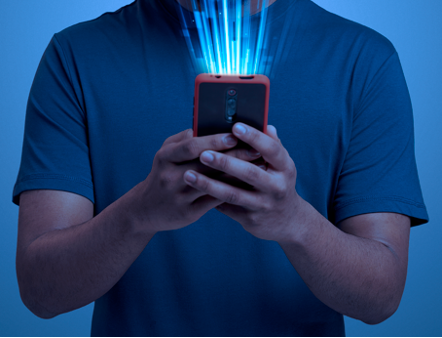
\includegraphics[width=0.4\textwidth]{imgs/fig.png}
\end{figure}

\textcolor{blue}{
Para construir um referencial teórico, o estudante deve revisar a literatura,
abordando conceitos fundamentais, trabalhos acadêmicos e/ou sistemas similares
ao seu estudo. É essencial incluir trabalhos relacionados, comparando
metodologias e identificando limitações, além de analisar outros sistemas
existentes, destacando suas funcionalidades e diferenciais. A organização do
referencial deve seguir uma progressão lógica, do geral para o específico,
demonstrando a lacuna na pesquisa e  justificando a relevância do estudo.
}

\section{Metologia}

\textcolor{blue}{
A Metodologia deve incluir o desenvolvimento do sistema, detalhando sua
implementação de forma clara e objetiva. Caso necessário, os requisitos
funcionais e não funcionais podem ser apresentados para contextualizar o
funcionamento do sistema e justificar as escolhas técnicas. Além disso,
recomenda-se a inclusão de um esquema ilustrativo da arquitetura do sistema,
facilitando a compreensão da sua estrutura e organização. Por fim, é essencial
descrever os métodos de verificação e/ou validação utilizados para garantir a
qualidade do sistema, especificando os critérios adotados para aferir os
aspectos desejados, como desempenho, segurança, usabilidade ou conformidade com
os requisitos definidos.
}

\section{Resultados e Discussão}

\textcolor{blue}{
A seção de Resultados e Discussão deve apresentar os dados obtidos na
verificação e/ou validação do sistema, destacando aqueles mais relevantes para
responder às perguntas e atender aos objetivos da pesquisa. A organização dos
resultados deve seguir uma ordem lógica, alinhada à Metodologia, garantindo
clareza na análise. Além de descrever os achados, essa seção deve interpretá-los
e relacioná-los ao referencial teórico, comparando-os com estudos anteriores
para identificar padrões, implicações e possíveis explicações. Gráficos, tabelas
e figuras podem ser utilizados para ilustrar as descobertas de forma objetiva e
facilitar a compreensão. Por fim, a discussão deve contextualizar os resultados,
apontando limitações do estudo, contribuições para a área e direções para
pesquisas futuras, sempre com embasamento nos dados apresentados.
}

\section{Considerações finais}

\textcolor{blue}{
As considerações finais deve destacar como o trabalho contribui para o avanço do
conhecimento na área, indo além da simples repetição do resumo ou listagem de
resultados. Essa seção deve apresentar uma justificativa científica clara,
indicando a relevância dos achados e suas possíveis aplicações ou extensões.
Além disso, é recomendado sugerir pesquisas futuras e experimentos
complementares que possam aprofundar os resultados obtidos. As conclusões podem
ser tanto gerais quanto específicas, sempre alinhadas aos objetivos
estabelecidos na introdução, garantindo uma síntese coerente e impactante do
estudo \cite{tanenbaum2023redes}.
}

\bibliography{referencias} % As referências serão formatadas de acordo com o estilo APA


\end{document}